\documentclass{article}
\usepackage{graphicx}

\textheight25cm
\topmargin-0.5cm
\pagestyle{empty}

\title {Algorithms and Games\\Homework 1}
\author {David Bulovic 11819382}
\date {}

\begin{document}
\maketitle

Matr.Nr.: \\
    $\begin{array}{*{8}{|p{16pt}}|}
    \hline
  1&1&8&1&9&3&8&2\\
    \hline
 $m_1$&$m_2$&$m_3$&$m_4$&$m_5$&$m_6$&$m_7$&$m_8$\\
    \hline
    \end{array}$ \\[3ex]
%
Node evaluation: \\
    $\begin{array}{*{8}{|p{16pt}}|}
    \hline
    -31&-32&37&-34&45&-16&33&-28\\
    \hline
    $x_1$&$x_2$&$x_3$&$x_4$&$x_5$&$x_6$&$x_7$&$x_8$\\
    \hline
    \end{array}$  \\[6ex]

\begin{figure}[h]
\center
	\hspace{6ex}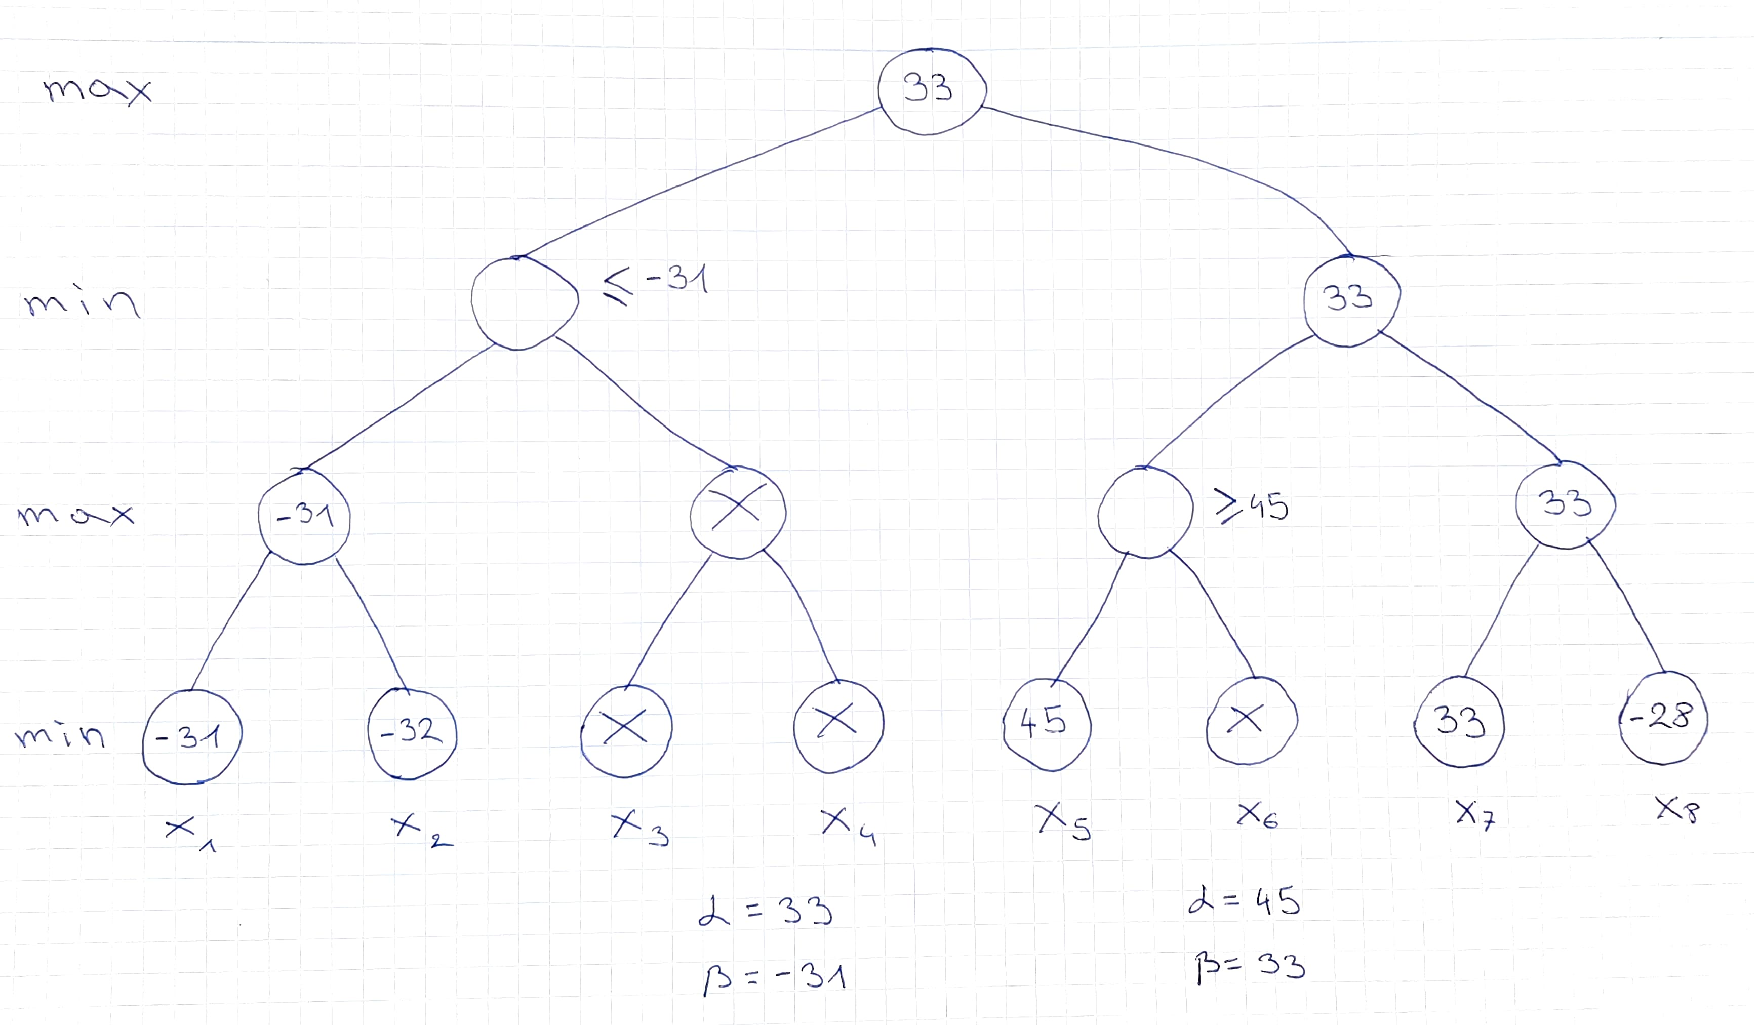
\includegraphics[width=\textwidth]{alpha}
\end{figure}

Nodes marked with 'X' are the ones that can be skipped. From x1 and x2 we get -31 in the maximizer above. Which means that the value in the minimizer
above cannot be larger than -31, which is always smaller than 33. This is why values of x3 and x4 are irrelevant, the outcome is always the same, regardless of them. \\ In the other part of the tree, x6 can be skipped, because the value in the 
maximizer above cannot be smaller than 45, which is always larger than 33, which will always be taken by the minimizer above that. Alpha and Beta values
are also noted below the graph.


\end{document}